% -*- coding:utf-8 -*-

\chapter{第三章}
\zhlipsum

\section{二级标题}
见脚注\footnote{\url{https://data.stats.gov.cn}}。
\zhlipsum

见表\ref{tab:example1}\zhlipsum[1]

\begin{table}[H]
  \small
  \caption{表格标题表格标题表格标题\label{tab:example1}}
  \adjustbox{center}{%
    \begin{tabular}{lrrrrrrrr}
      \toprule
               & \multicolumn{1}{l}{内容} & \multicolumn{1}{l}{内容} & \multicolumn{1}{l}{内容} & \multicolumn{1}{l}{内容} & \multicolumn{1}{l}{内容} & \multicolumn{1}{l}{内容} & \multicolumn{1}{l}{内容} & \multicolumn{1}{l}{内容} \\
      \midrule
      表格内容 & 123                      & 4.56                     & 7.89                     & 5.67                     & 7.89                     & 1.23                     & -4.56                    & 7.89                     \\
      表格内容 & 123                      & 4.56                     & 7.89                     & 5.67                     & 7.89                     & 10.23                    & 2.38                     & 11.64                    \\
      \bottomrule
    \end{tabular}}%
  \vspace{1.5ex}
  \begin{minipage}{\textwidth}
    \phantom{缩进}注:如有需要可对表格进行注释说明,可省略。
    如有需要可对表格进行注释说明,可省略。
    如有需要可对表格进行注释说明,可省略。\\
    \phantom{缩进}数据来源:如需对数据来源进行说明,请参照此格式,可省略。
    如需对数据来源进行说明,请参照此格式,可省略。
  \end{minipage}
\end{table}%
\vspace{-3ex}
\zhlipsum

\subsection{三级标题}
\zhlipsum*[2] 正文正文正文见图\ref{fig:CO_2}。

\begin{figure}[H]
  \adjustbox{center}{%
    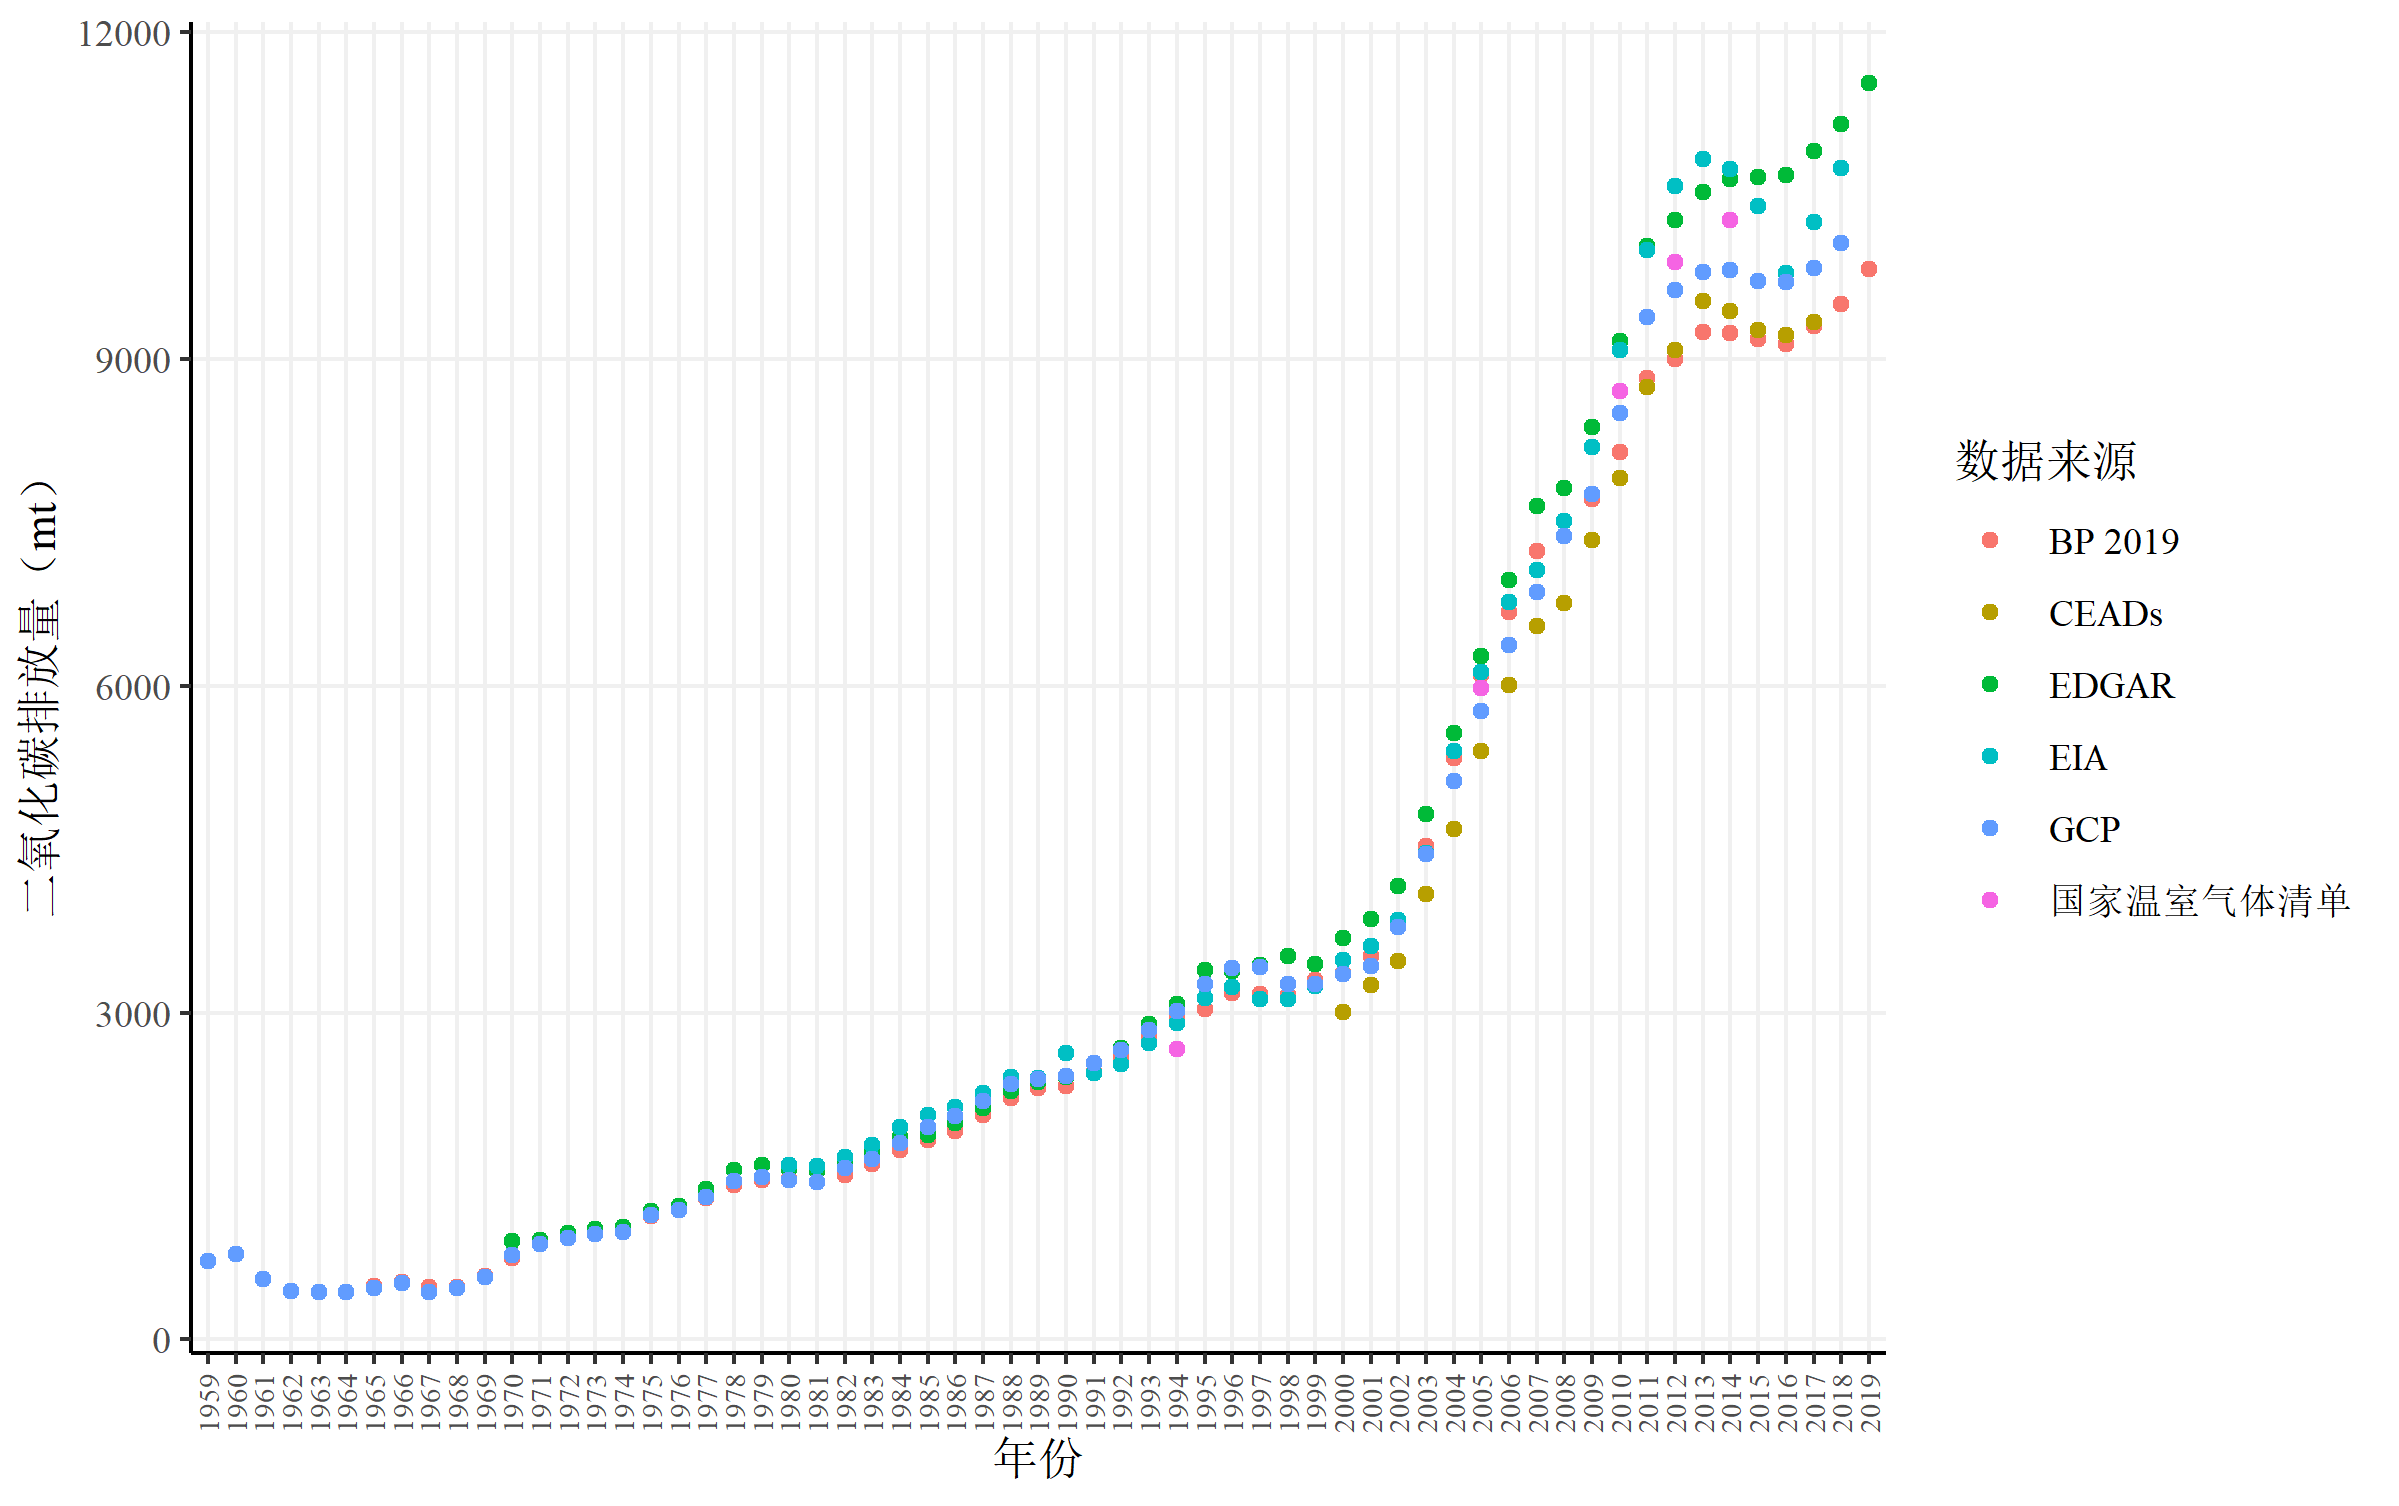
\includegraphics[width=5in]{emission.png}}
  \caption{中国1959-2019年二氧化碳排放量\label{fig:CO_2}}
\end{figure}

见图\ref{fig:side_1}。\zhlipsum[1]
\hvFloat[%
  capPos=bottom,
  rotAngle=-90,
  objectPos=center]%
{figure}{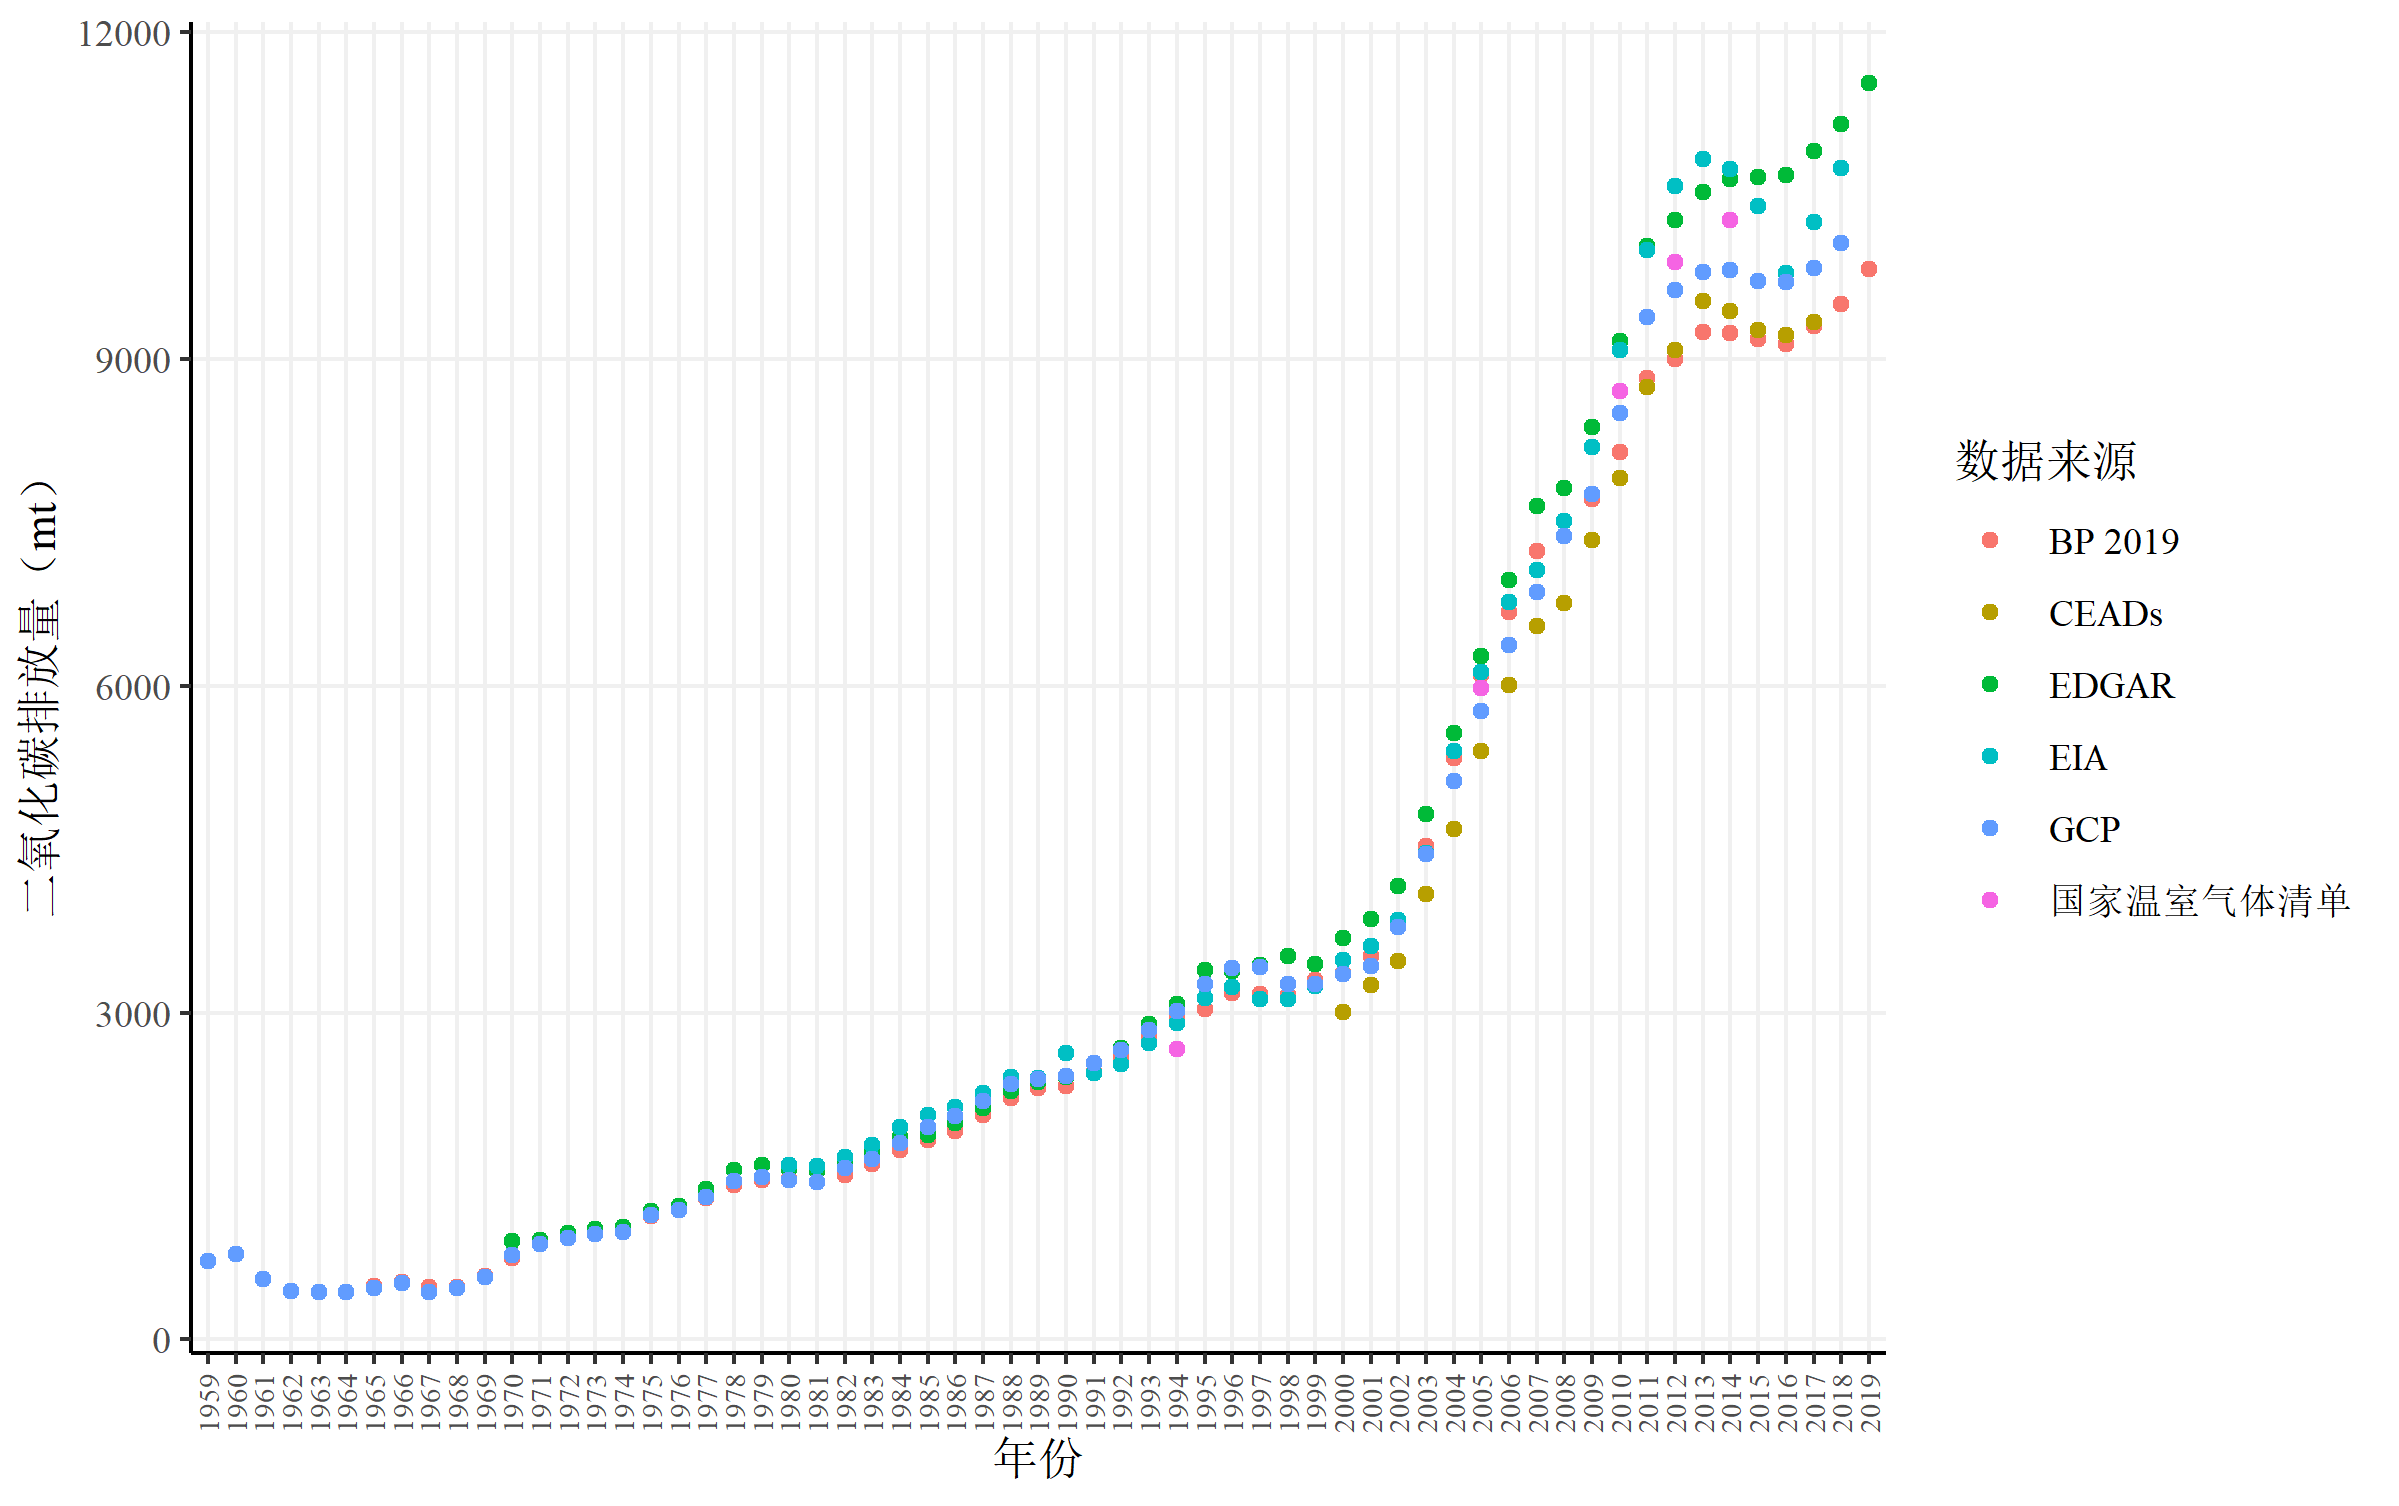
\includegraphics[width=5in]{emission.png}}
{中国1959-2019年二氧化碳排放量}{fig:side_1}
\vspace{-5ex}
\zhlipsum* 见图\ref{fig:side_2}。

\hvFloat[%
  capPos=bottom,
  rotAngle=90,
  objectPos=center]%
{figure}{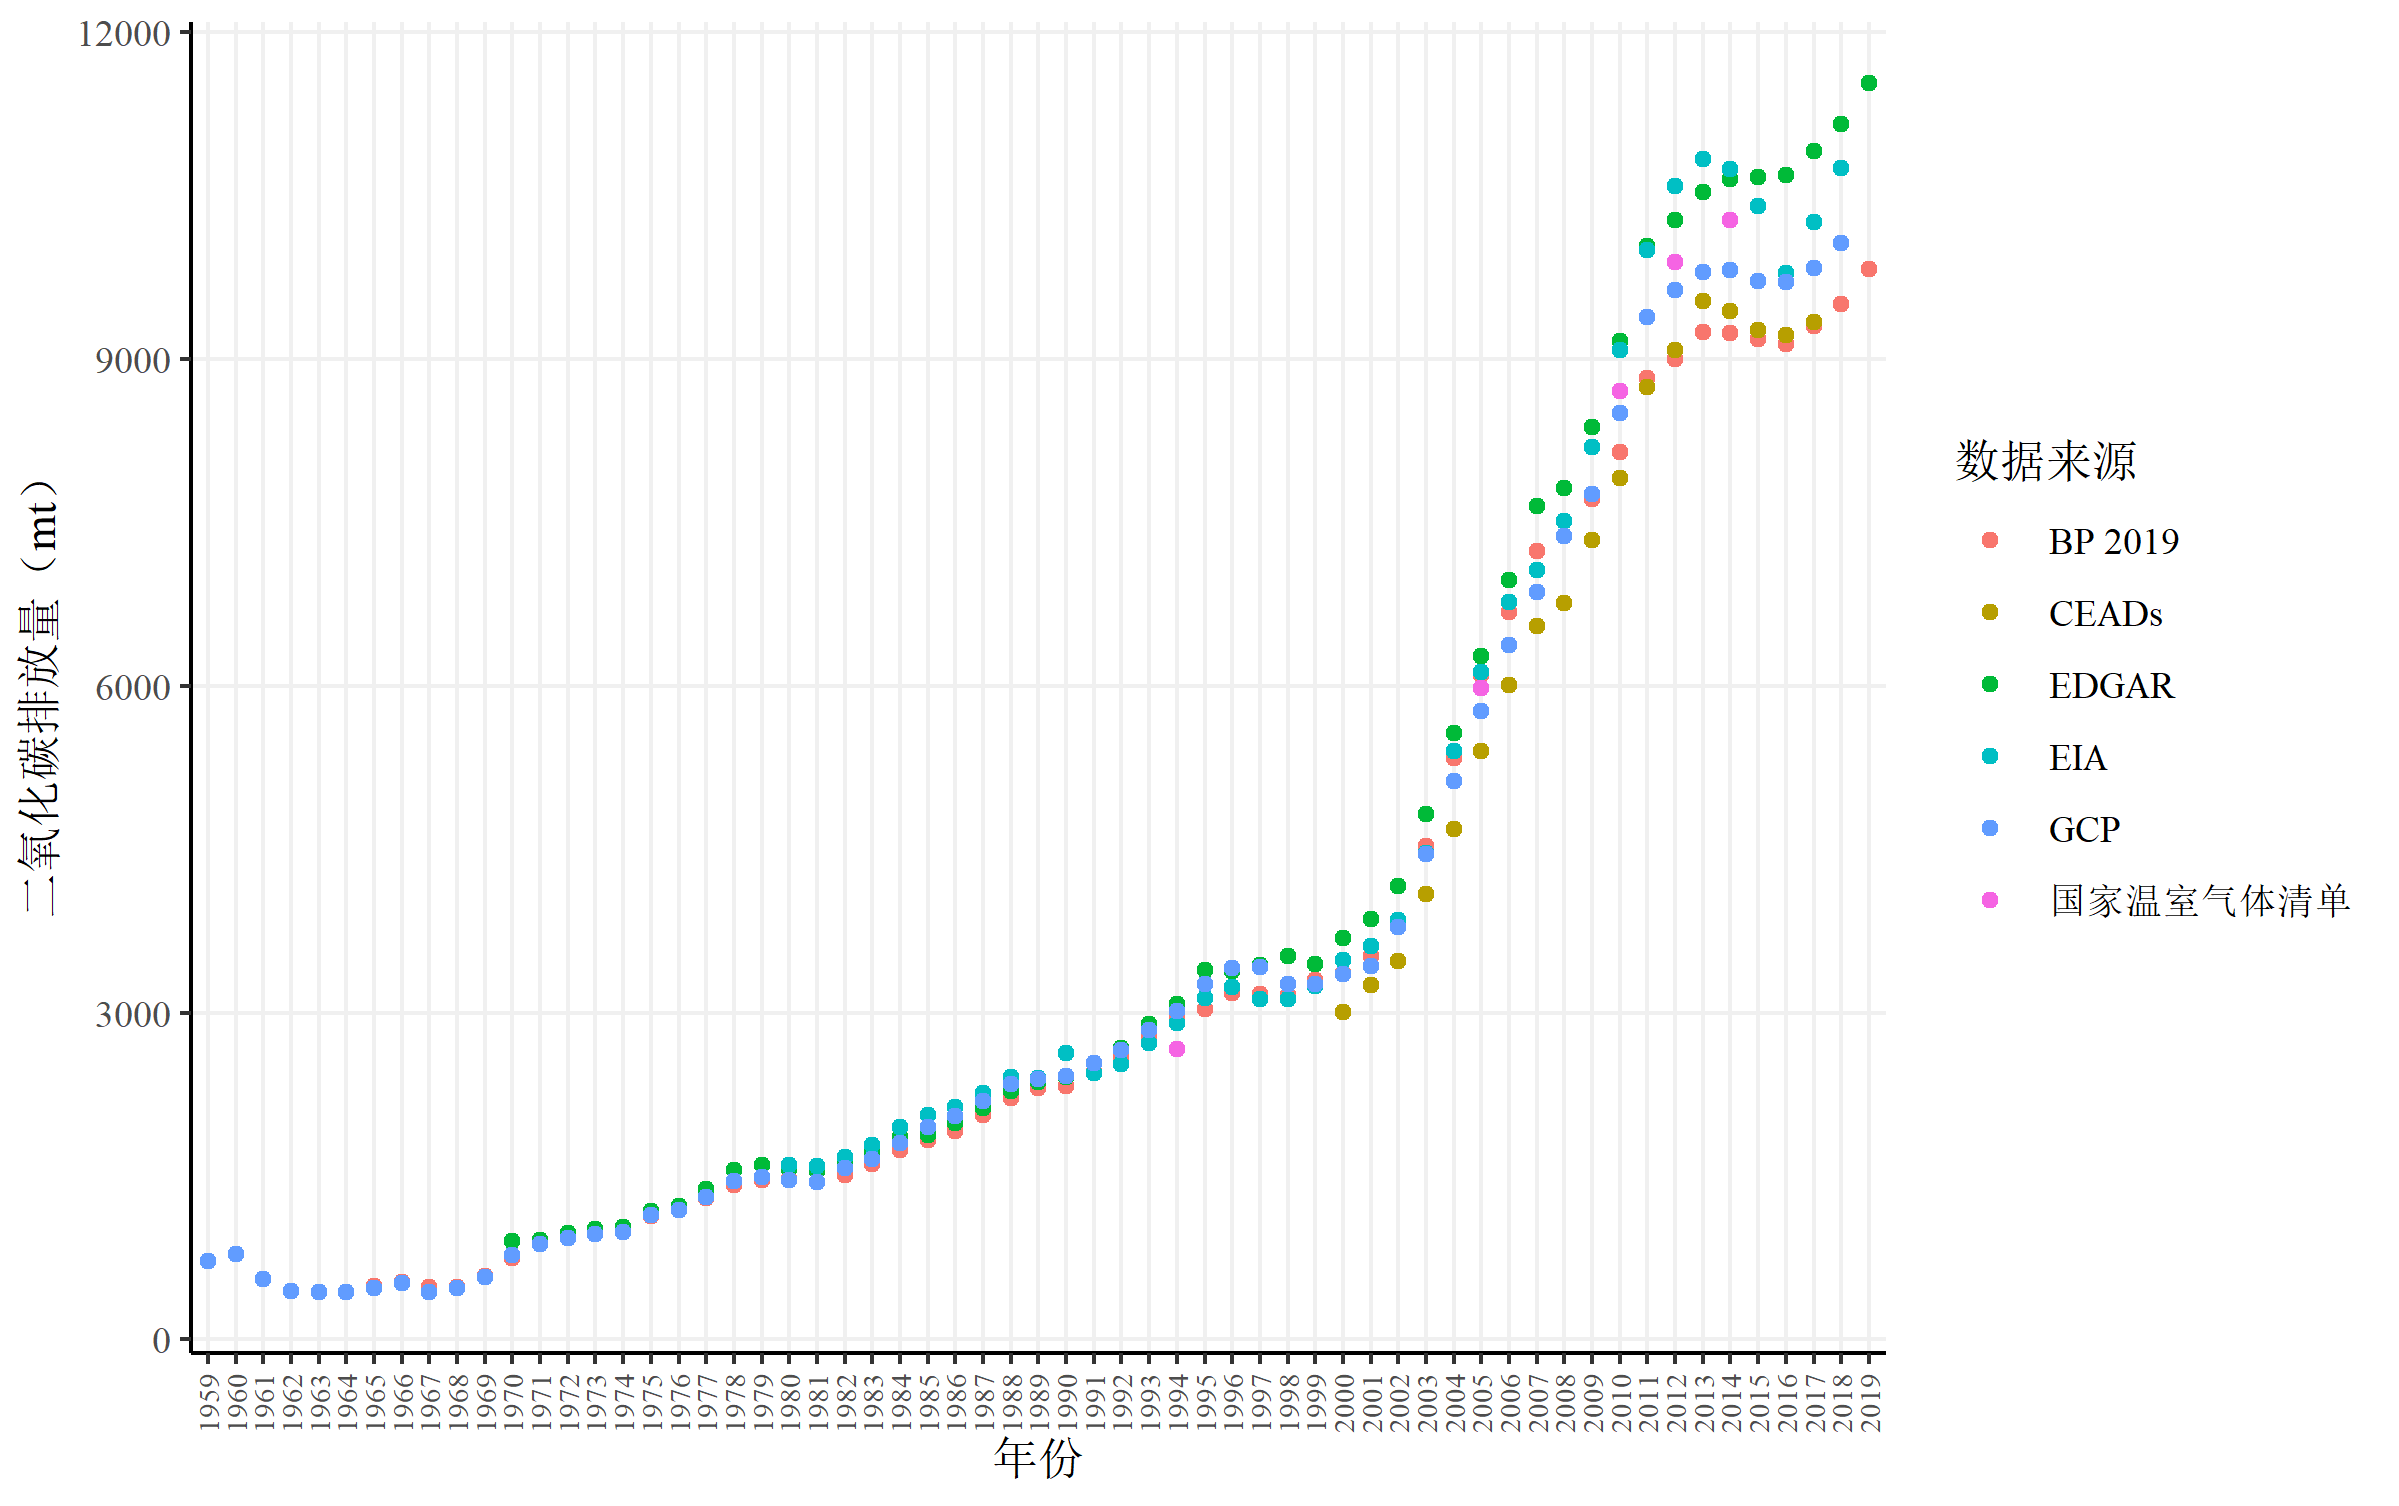
\includegraphics[width=5in]{emission.png}}
{中国1959-2019年二氧化碳排放量}{fig:side_2}
\vspace{-5ex}
\zhlipsum*
正文正文正文正文(见表\ref{tab:side_1}和表\ref{tab:side_2})。
\zhlipsum[1]

\savebox{\hvOBox}{%
  \small
  %\renewcommand{\arraystretch}{0.8} % 如果横置还是超宽,可以适当缩小表格行间距
  \begin{tabular}{llrrrrrrrrrrrr}
    \toprule
    \multirow{2}[4]{*}{变量}                       & \multirow{2}[4]{*}{变量变量}   & \multicolumn{1}{c}{\multirow{2}[4]{*}{变量}} & \multicolumn{5}{c}{变量} & \multicolumn{5}{c}{变量} & \multicolumn{1}{c}{\multirow{2}[4]{*}{变量}}                                                                                                                                                                                                     \\
    \cmidrule{4-13}                                &                                &                                              & \multicolumn{1}{c}{0}    & \multicolumn{1}{c}{1}    & \multicolumn{1}{c}{2}                        & \multicolumn{1}{c}{3} & \multicolumn{1}{c}{4} & \multicolumn{1}{c}{0} & \multicolumn{1}{c}{1} & \multicolumn{1}{c}{2} & \multicolumn{1}{c}{3} & \multicolumn{1}{c}{4} &                           \\
    \midrule
    \multirow{6}[2]{*}{正文正文}                   & 正文正文                       & 0.01                                         & 0.01                     & 0.01                     & 0.01                                         & 0.01                  & 0.01                  & 0.01                  & 0.01                  & 0.01                  & 0.01                  & 0.01                  & \multicolumn{1}{c}{0.01}  \\
                                                   & 正文正                         & 0.01                                         & 0.01                     & 0.01                     & 0.01                                         & 0.01                  & 0.01                  & 0.01                  & 0.01                  & 0.01                  & 0.01                  & 0.01                  & \multicolumn{1}{c}{0.01}  \\
                                                   & 正文正文                       & 0.01                                         & 0.01                     & 0.01                     & 0.01                                         & 0.01                  & 0.01                  & 0.01                  & 0.01                  & 0.01                  & 0.01                  & 0.01                  & \multicolumn{1}{c}{0.01}  \\
                                                   & 正文正正文                     & 0.01                                         & 0.01                     & 0.01                     & 0.01                                         & 0.01                  & 0.01                  & 0.01                  & 0.01                  & 0.01                  & 0.01                  & 0.01                  & \multicolumn{1}{c}{0.01}  \\
                                                   & 正文正文正文正文正文正文正文   & 0.01                                         & 0.01                     & 0.01                     & 0.01                                         & 0.01                  & 0.01                  & 0.01                  & 0.01                  & 0.01                  & 0.01                  & 0.01                  & \multicolumn{1}{c}{0.01}  \\
                                                   & 正文、正文正正文               & 0.01                                         & 0.01                     & 0.01                     & 0.01                                         & 0.01                  & 0.01                  & 0.01                  & 0.01                  & 0.01                  & 0.01                  & 0.01                  & \multicolumn{1}{c}{0.01}  \\
    \cmidrule{1-2}    \multirow{6}[2]{*}{正文正文} & 正文正正文                     & 0.01                                         & 0.01                     & 0.01                     & 0.01                                         & 0.01                  & 0.01                  & 0.01                  & 0.01                  & 0.01                  & 0.01                  & 0.01                  & \multicolumn{1}{c}{0.01}  \\
                                                   & 正文正正文正文正文             & 0.01                                         & 0.01                     & 0.01                     & 10.01                                        & 11.01                 & 0.01                  & 0.01                  & 10.01                 & 10.01                 & 10.01                 & 10.01                 & \multicolumn{1}{c}{0.01}  \\
                                                   & 正文正正文正文正正文           & 10.01                                        & 10.01                    & 0.01                     & 10.01                                        & 10.01                 & 0.01                  & 10.01                 & 10.01                 & 10.01                 & 10.01                 & 10.01                 & \multicolumn{1}{c}{0.01}  \\
                                                   & 正文正文正文正正文             & 0.01                                         & 0.01                     & 0.01                     & 0.01                                         & 10.01                 & 0.01                  & 0.01                  & 0.01                  & 0.01                  & 0.01                  & 0.01                  & \multicolumn{1}{c}{1.18 } \\
                                                   & 正文正文正文正文正文正文正文正 & 0.01                                         & 0.01                     & 0.01                     & 0.01                                         & 0.01                  & 0.01                  & 0.01                  & 0.01                  & 0.01                  & 0.01                  & 0.01                  & \multicolumn{1}{c}{0.01}  \\
                                                   & 正文正文正文正文正文正文正文   & 0.01                                         & 0.01                     & 0.01                     & 0.01                                         & 0.01                  & 0.01                  & 0.01                  & 0.01                  & 0.01                  & 0.01                  & 0.01                  & 0.01                      \\
    \bottomrule
  \end{tabular}%
}
\hvFloat[%
  floatPos=hb,
  useOBox=true,
  objectAngle=-90,
  capAngle=-90,
  capPos=right,
  capWidth=w]%
{table}{}{超宽表格横置示例}{tab:side_1}

\savebox{\hvOBox}{%
  \small
  %\renewcommand{\arraystretch}{0.8} % 如果横置还是超宽,可以适当缩小表格行间距
  \begin{tabular}{llrrrrrrrrrrrr}
    \toprule
    \multirow{2}[4]{*}{变量}                       & \multirow{2}[4]{*}{变量变量}   & \multicolumn{1}{c}{\multirow{2}[4]{*}{变量}} & \multicolumn{5}{c}{变量} & \multicolumn{5}{c}{变量} & \multicolumn{1}{c}{\multirow{2}[4]{*}{变量}}                                                                                                                                                                                                     \\
    \cmidrule{4-13}                                &                                &                                              & \multicolumn{1}{c}{0}    & \multicolumn{1}{c}{1}    & \multicolumn{1}{c}{2}                        & \multicolumn{1}{c}{3} & \multicolumn{1}{c}{4} & \multicolumn{1}{c}{0} & \multicolumn{1}{c}{1} & \multicolumn{1}{c}{2} & \multicolumn{1}{c}{3} & \multicolumn{1}{c}{4} &                           \\
    \midrule
    \multirow{6}[2]{*}{正文正文}                   & 正文正文                       & 0.01                                         & 0.01                     & 0.01                     & 0.01                                         & 0.01                  & 0.01                  & 0.01                  & 0.01                  & 0.01                  & 0.01                  & 0.01                  & \multicolumn{1}{c}{0.01}  \\
                                                   & 正文正                         & 0.01                                         & 0.01                     & 0.01                     & 0.01                                         & 0.01                  & 0.01                  & 0.01                  & 0.01                  & 0.01                  & 0.01                  & 0.01                  & \multicolumn{1}{c}{0.01}  \\
                                                   & 正文正文                       & 0.01                                         & 0.01                     & 0.01                     & 0.01                                         & 0.01                  & 0.01                  & 0.01                  & 0.01                  & 0.01                  & 0.01                  & 0.01                  & \multicolumn{1}{c}{0.01}  \\
                                                   & 正文正正文                     & 0.01                                         & 0.01                     & 0.01                     & 0.01                                         & 0.01                  & 0.01                  & 0.01                  & 0.01                  & 0.01                  & 0.01                  & 0.01                  & \multicolumn{1}{c}{0.01}  \\
                                                   & 正文正文正文正文正文正文正文   & 0.01                                         & 0.01                     & 0.01                     & 0.01                                         & 0.01                  & 0.01                  & 0.01                  & 0.01                  & 0.01                  & 0.01                  & 0.01                  & \multicolumn{1}{c}{0.01}  \\
                                                   & 正文、正文正正文               & 0.01                                         & 0.01                     & 0.01                     & 0.01                                         & 0.01                  & 0.01                  & 0.01                  & 0.01                  & 0.01                  & 0.01                  & 0.01                  & \multicolumn{1}{c}{0.01}  \\
    \cmidrule{1-2}    \multirow{6}[2]{*}{正文正文} & 正文正正文                     & 0.01                                         & 0.01                     & 0.01                     & 0.01                                         & 0.01                  & 0.01                  & 0.01                  & 0.01                  & 0.01                  & 0.01                  & 0.01                  & \multicolumn{1}{c}{0.01}  \\
                                                   & 正文正正文正文正文             & 0.01                                         & 0.01                     & 0.01                     & 10.01                                        & 11.01                 & 0.01                  & 0.01                  & 10.01                 & 10.01                 & 10.01                 & 10.01                 & \multicolumn{1}{c}{0.01}  \\
                                                   & 正文正正文正文正正文           & 10.01                                        & 10.01                    & 0.01                     & 10.01                                        & 10.01                 & 0.01                  & 10.01                 & 10.01                 & 10.01                 & 10.01                 & 10.01                 & \multicolumn{1}{c}{0.01}  \\
                                                   & 正文正文正文正正文             & 0.01                                         & 0.01                     & 0.01                     & 0.01                                         & 10.01                 & 0.01                  & 0.01                  & 0.01                  & 0.01                  & 0.01                  & 0.01                  & \multicolumn{1}{c}{1.18 } \\
                                                   & 正文正文正文正文正文正文正文正 & 0.01                                         & 0.01                     & 0.01                     & 0.01                                         & 0.01                  & 0.01                  & 0.01                  & 0.01                  & 0.01                  & 0.01                  & 0.01                  & \multicolumn{1}{c}{0.01}  \\
                                                   & 正文正文正文正文正文正文正文   & 0.01                                         & 0.01                     & 0.01                     & 0.01                                         & 0.01                  & 0.01                  & 0.01                  & 0.01                  & 0.01                  & 0.01                  & 0.01                  & 0.01                      \\
    \bottomrule
  \end{tabular}%
}
\hvFloat[%
  floatPos=hb,
  useOBox=true,
  objectAngle=90,
  capAngle=90,
  capPos=left,
  capWidth=w]%
{table}{}{超宽表格横置示例}{tab:side_2}








